\section{Quantum Capacity of Quantum Channels}

\begin{frame}{Quantum Capacity of a Quantum Channel}
The quantity capacity $Q(\mathcal{N})$ of a quantum channel is defined as follows (where $\ket{\psi} = U^{\mathcal{N}}_{A' \rightarrow BE} \ket{\phi}_{AA'}$).
\begin{tcolorbox}
$$Q(\mathcal{N}) = \max_{\phi_{AA'}} \left[ S(B)_\rho - S(AB)_\rho \right]$$
\end{tcolorbox}

\begin{figure}
    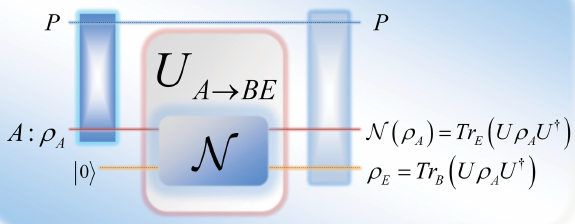
\includegraphics[width=0.5\textwidth]{figures/quantum_communication_quantum_channel.png}
    \caption{Quantum communication through a quantum channel \cite{Gyongyosi_2018}.}
\end{figure}
\end{frame}

\begin{frame}{Properties: Quantum Capacity of a Quantum Channel}
\begin{itemize}
    \setlength{\itemsep}{1.5em}
    \item Non-negativity
    $$Q(\mathcal{N}) \geq 0$$
    \item Non-additivity
    $$Q(\mathcal{N} \otimes \mathcal{M}) \neq Q(\mathcal{N}) + Q(\mathcal{M})$$
    \item Relation with other capacities
    $$Q(\mathcal{N}) \leq P(\mathcal{N}) \leq C(\mathcal{N})$$
\end{itemize}
\end{frame}

\begin{frame}{Degradable Quantum Channels}
A channel $\mathcal{N}: \mathcal{H}_A \rightarrow \mathcal{H}_B$ is called degradable when it may be degraded to its complementary channel $\mathcal{N}^c: \mathcal{H}_A \rightarrow \mathcal{H}_E$, i.e. when there exists a CPTP map $T: \mathcal{H}_B \rightarrow \mathcal{H}_E$ such that
\begin{tcolorbox}
\begin{align*}
\mathcal{N}^c = T \circ \mathcal{N}
\end{align*}
\end{tcolorbox}

\begin{figure}
    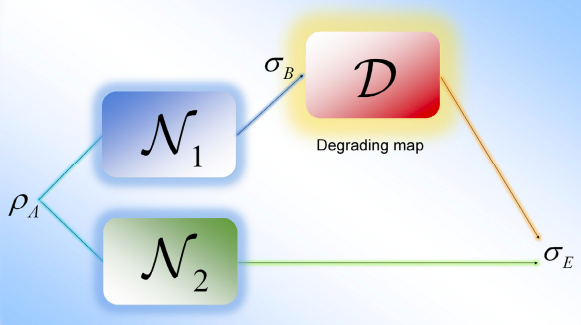
\includegraphics[width=0.4\textwidth]{figures/degradable_quantum_channel.png}
    \caption{The concept of a degradable quantum channel \cite{Gyongyosi2012PropertiesOT}.}
\end{figure}
\end{frame}

\begin{frame}{Properties: Degradable Quantum Channels}
\begin{itemize}
    \setlength{\itemsep}{1.5em}
    \item Additivity of Private Capacity
    $$P(\mathcal{N} \otimes \mathcal{M}) = P(\mathcal{N}) + P(\mathcal{M})$$
    \item Additivity of Quantum Capacity
    $$Q(\mathcal{N} \otimes \mathcal{M}) = Q(\mathcal{N}) + Q(\mathcal{M})$$
    \item Equivalence of Private and Quantum Capacity
    $$Q(\mathcal{N}) = P(\mathcal{N})$$
\end{itemize}
\end{frame}
